\section{Cxense}
\label{sec:cxense}
%Our project is a collaboration project between \emph{University of Oslo} and \emph{Cxense}, where Cxense provids lost of th



Cxense is a software company that collects and analyzes online information about Internet users. This information is used to create content profiles and user profiles, which can be used to understand the Internet activity. Their main goal is to understand the user's interest. Cxense provides software for companies, including tools to provide advertising, user recommendations and targeting emails \cite{aboutcxense}.

This project is a collaboration project between University of Oslo and Cxense. Thus, Cxense's software is used in our process of categorizing texts. Figure \ref{fig:categorization_figure} illustrates the complete categorization process of the keywords. When this process is complete, we have a list of categorized keywords which is needed for categorizing any input text. Cxense's software is part of our classifier in the process of finding keywords within the text. 
\begin{figure}[h]
\centering

\includegraphics[width=\textwidth]{Chapters/Background/Categorization_figure}
\caption[The categorization process of the keywords]{Illustration of the categorization process of the keywords.}
\label{fig:categorization_figure}
\end{figure}

There are different ways of finding the keywords in a text. Figure \ref{fig:cxensematching} illustrates the general approach where the whole dictionary is intersected with the document, and the result is a list of all entries found in both the dictionary and the document. 

\begin{figure}[h]
\centering
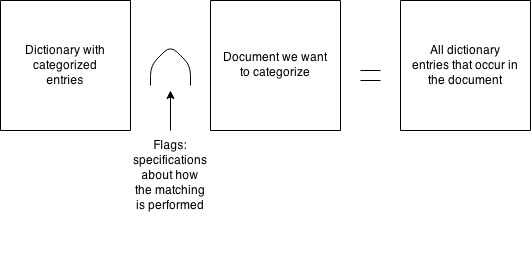
\includegraphics[width=\textwidth]{Chapters/Background/Cxense_matching}
\caption[Illustration of entry matching process]{Illustration of the categorization of a text, where the classifier finds all dictionary entries that occur in the text. }
\label{fig:cxensematching}
\end{figure}

Cxense's software allows the user to specify how the matching should occur. This is done by adding flags (specifications) in the intersection process. We have chosen to use exact matching in our project which means that the words have to be identical to be considered a match. We have also chosen to use case insensitivity (words in lower case can be identical match to words in upper case) and normalization of the words. The normalization of the words were to make sure all words were in the same character encoding. 

It is also possible to decide the lower limit of keyword occurrences from a category before the class is assigned to an article. This is done by creating weights of the keywords' classes and can be used to optimize the classifier.

%normalized text. 


%Det er “overlap” mode som brukes, typisk case-insensitivt (se “key-normalization-flags”), og “count” og “unique-count” styrer en precision/recall tradeoff. Ja, det er eksakt matching (modulo “key-normalization-flags”) og ikke matching på lemmatiserte verdier — vi har en opsjon for det siste også, men den er ikke dokumentert. Som default er vel “leftmost-longest-matching” true, IIRC.